\chapter{フェルミオンの符号と超対称性による相殺}

\lectureoverview{超対称性はボソンとフェルミオンを関係づけるが、そのような関係を望む理由は、その代数を書き下す前に見る方が容易である。まず回転の位相幾何学から始め、フェルミオン波動関数の符号を干渉を通じて観測可能にし、閉じたフェルミオンループのマイナス符号を交換反対称性から導き、次にボソンループとフェルミオンループの逆符号を用いて真空エネルギーとスカラー自己エネルギーの相殺を動機づける。後半では、超対称性がどの程度まで破れうるか、超対称パートナーをどのように検出しうるか、そして厳密な超対称性がなぜ通常の原子殻構造を消し去るのかを問う。}

\section{超対称性以前：回転の奇妙な性質}

超対称性はフェルミオンとボソンの間の対称性である。しかしそれを構成しようとする前に、これら二種類の粒子が回転に対してどれほど異なって応答するかを思い出す価値がある。その問い自体は、実演が容易でありながら、一度見てしまうと忘れるのが驚くほど難しい位相幾何学的事実から始まる。

片手を手のひらを上にして持ち、手首を\(2\pi\)回転させる。手は元の向きに戻るが、腕は明らかに等価な配置には戻っていない。腕はねじれている。必要に応じて腕を動かしながら、さらに\(2\pi\)回転させ続けると、そのねじれは取り除ける。したがって、周囲を固定したままでは\(2\pi\)回転は回転なしへ連続的に変形できないが、\(4\pi\)回転は変形できる。この手の実演は、最も文字通りの意味での手振りによる証明である。

同じ点は解剖学に頼らずに示すこともできる。固定された箱の中に球を置き、その球を、柔軟で伸縮可能だが切れない任意の本数のひもで壁に結びつける。球を\(2\pi\)回転させる。ひもは絡まり、ひもだけをどのように動かしても元の配置には戻せない。球を合計\(4\pi\)回転させると、ひもを球の周りに巡らせて絡まりを消すことができる。壁は空間的無限遠を表す。この比較が意味をもつのは、境界が球とともに回転されないからにほかならない。

\begin{classroomqa}
\audiencequestion{箱を回転させれば絡まりを取り除けるのではないか。\lecturetimestamp{00:02:53}}
\lecturerresponse{それは問題を変えてしまう。箱は空間的無限遠を表しており、固定されている。我々は物体と周囲の共通の回転ではなく、周囲に対する物体の回転を比較しているのである。}
\end{classroomqa}

\begin{classroomqa}
\audiencequestion{なぜ単に球をもう\(2\pi\)回転させないのか。\lecturetimestamp{00:03:20}}
\lecturerresponse{まさにそれが二つの場合を区別する。球をさらに回転させなければ、\(2\pi\)回転で生じた絡まりは取り除けない。二回目の回転の後、合計\(4\pi\)になれば、取り除ける。}
\end{classroomqa}

現代の群の言葉では、回転群は閉じた経路の二つの位相幾何学的類をもつ：
\begin{equation}
\pi_1\!\left(SO(3)\right)\cong \mathbb Z_2.
\end{equation}
一回の周回は非自明であるが、二回周回すると自明な類を与える。
等価に、\(SU(2)\)は\(SO(3)\)の二重被覆である。これがフェルミオン符号の幾何学的先史である。

\editorialnote{\(SO(3)\)、\(SU(2)\)、および基本群の言葉が位相幾何学を明示する。腕の実演とひもの実演は、同じ二値的振る舞いを幾何学的に確立する。}

\section{\texorpdfstring{\(2\pi\)}{2 pi}回転が量子状態に何をするか}

ここで粒子の位置を固定し、そのスピン状態のみを保持し、それを\(\ket{\psi}\)で表す。整数スピンの粒子はボソンであり、半整数スピンの粒子はフェルミオンである。物理的回転は、荷電スピンを強い磁場中に置いて磁場を回転させることによって、あるいは固定磁場中でスピンを所望の角度だけ歳差運動させることによって実現できる。

\begin{classroomqa}
\audiencequestion{実験室で電子スピンを実際にどのように回転させられるのか。\lecturetimestamp{00:05:26}}
\lecturerresponse{磁場が取っ手を与える。十分に強い磁場を回転させてスピンをそれに追随させるか、固定磁場の周りでスピンを歳差運動させればよい。電子を手でつかむのは競争力のある実験方法ではない。}
\end{classroomqa}

完全な\(2\pi\)回転が状態を位相倍するものとせよ：
\begin{equation}
R(2\pi)\ket{\psi}=\xi\ket{\psi}.
\end{equation}
この操作を二度行うと
\begin{equation}
R(4\pi)\ket{\psi}=\xi^2\ket{\psi}.
\end{equation}
\(4\pi\)経路は位相幾何学的に自明であるから、この比較では恒等操作として作用しなければならない。したがって
\begin{equation}
\xi^2=1,
\qquad
\xi=+1\ \hbox{or}\ -1.
\end{equation}
ボソンはプラス符号を実現し、フェルミオンはマイナス符号を実現する：
\begin{align}
R(2\pi)\ket{\psi_B}&=+\ket{\psi_B},\\
R(2\pi)\ket{\psi_F}&=-\ket{\psi_F}.
\end{align}
確定したスピン\(j\)の状態に対しては、簡潔な表現は
\begin{equation}
R(2\pi)=(-1)^{2j}.
\end{equation}
記録は第二の可能性が\(2\pi\)の掛け算であると簡単に述べているが、周囲の導出と板書の議論から、意図された因子は\(-1\)であることが明らかである。

一見すると、これは物理的に空虚に思える。波動関数全体が符号を変えるなら、
\begin{equation}
\Psi\longmapsto-\Psi,
\end{equation}
確率は変わらない。なぜなら
\begin{equation}
(-\Psi)^*(-\Psi)=\Psi^*\Psi.
\end{equation}
だからである。同一に準備された電子の集団を二つ用意し、一方の集団のすべてのメンバーを\(2\pi\)回転させ、他方の集団はそのままにしておく。孤立したメンバーに対するいかなる測定も、それがどちらの集団に由来するかを明らかにできない。全体位相は観測量ではない。

\section{負号を相対的なものにする}

符号は、波動関数の一方のコヒーレントな枝に課され、他方には課されないときに観測可能になる。電子を一度に一つずつ二経路装置に送る。どちらの経路を通ったかを決定してはならない。なぜなら、経路情報は干渉を破壊するからである。上側と下側の振幅を\(\psi_1\)と\(\psi_2\)とすると、再結合後の状態は
\begin{equation}
\Psi=\psi_1+\psi_2.
\end{equation}
となる。各枝を一時的に磁場領域に閉じ込めると想像する。第二の枝に対応する磁場だけを\(2\pi\)回転させる。粒子がフェルミオンなら、状態は
\begin{equation}
\Psi'=\psi_1-\psi_2.
\end{equation}
となる。これはもはや全体符号ではない。相対位相は干渉の極大を極小へ移す。戻ってくる二つの波束が検出器の中央に関して鏡像なら、反対称な組み合わせは中心で消える：
\begin{equation}
\Psi'(0)=\psi_1(0)-\psi_2(0)=0.
\end{equation}
したがって電子はその対称点で決して検出されない。両方の枝を回転させれば代わりに\(-\psi_1-\psi_2=-\Psi\)が得られるが、これは観測可能な効果を持たない。

講義はこの実験の関係的な性質を強調する。一方の磁場領域をもう一方に対して回転させることは、箱を固定したまま球を回転させることに類似する。両方の領域を一緒に回転させることは、球と箱を一緒に回転させることに類似する。相対的な\(4\pi\)回転は効果を取り除く。なぜなら、フェルミオン状態はそのときプラス符号で戻るからである。この実験は1967年にヤキール・アハラノフとレナード・サスキンドによって提案され、後に干渉計の形で実現されたと、講義はついでに述べている。同じ原理は電子や荷電イオンに適用できる。ずれた縞模様は半整数スピン状態を同定し、ずれていない縞模様は整数スピン状態を同定する。

\begin{classroomqa}
\audiencequestion{相対磁場を\(4\pi\)回転させると、ずれた縞模様は元の縞模様に戻るか？\lecturetimestamp{00:12:21}}
\lecturerresponse{はい。二つの符号変化は掛け合わさって\(+1\)になるので、極大と極小を交換する原因である相対位相は消える。}
\end{classroomqa}

\begin{classroomqa}
\audiencequestion{箱の中のひもは、どの程度文字通りにフェルミオンと結びつけられるべきか？\lecturetimestamp{00:13:43}}
\lecturerresponse{それらは位相幾何学的な記憶補助であり、電子に付着した物理的なひもではない。ボソンは\(2\pi\)回転が記憶を残さないかのように振る舞い、フェルミオンは非自明なもつれによって表される符号の記憶を正確に保持する。}
\end{classroomqa}

\begin{classroomqa}
\audiencequestion{二つの磁場領域に二つの電子があり、一方が回転され、他方は回転されていないのか？\lecturetimestamp{00:14:29}}
\lecturerresponse{いいえ。コヒーレントな空間的重ね合わせの中に一つの電子がある。それはどちらの枝を占めるかという振幅を持ち、装置はどちらの枝を占めたかを明らかにしてはならない。一方の領域を回転させると一方の振幅が他方に対して変化し、両方を回転させると共通位相だけが変化する。}
\end{classroomqa}

角度\(2\pi\)が特別なのは、スピンの向きがそれ自身に戻る一方でスピノルが符号を獲得するからである。一般的な相対回転はスピンの向きも変える。二つの経路状態がスピン状態\(\ket{\chi_1}\)と\(\ket{\chi_2}\)で戻るなら、干渉項は
\begin{equation}
\braket{\chi_1}{\chi_2}.
\end{equation}
に比例する。その大きさが縞の可視度を制御する。\editorialnote{スピン重なり公式は、干渉の部分的および完全な消失に関する講義の定性的議論を標準的に補完するものである。}直交するスピン状態は完全な経路情報を持ち、干渉しない。

\begin{classroomqa}
\audiencequestion{どちらの磁場領域に電子が含まれていたかを測定するとどうなるか？\lecturetimestamp{00:18:03}}
\lecturerresponse{干渉縞は破壊される。二つの経路を区別するいかなる記録も、それらの振幅のコヒーレントな足し合わせを取り除く。}
\end{classroomqa}

\begin{classroomqa}
\audiencequestion{すべてのスピンが同じ向きから始まり、最終スピンが測定されるなら、\(2\pi\)操作自体がその向きを変えるのか？\lecturetimestamp{00:18:17}}
\lecturerresponse{いいえ。\(2\pi\)の後、物理的なスピンの向きは同じである。フェルミオン的な枝だけが負号を獲得したのである。だからこそこの操作は、異なるスピンの向きを経路の目印として残すことなく、干渉を変えうるのである。}
\end{classroomqa}

\begin{classroomqa}
\audiencequestion{場が\(2\pi\)ではなく\(\pi\)だけ回されたらどうなるか？\lecturetimestamp{00:18:43}}
\lecturerresponse{その場合、スピンの向きが変わる。上向きスピン分枝と下向きスピン分枝は区別可能であり、干渉できない。中間の角度では可視度が連続的に低下し、\(180^\circ\)の相対回転で完全に消失する。}
\end{classroomqa}

\section{交換対称性と閉ループの符号}

回転の議論は一つのフェルミオン的マイナス符号を孤立させた。同一粒子の交換の際には、密接に関連する第二の符号が現れる。二粒子波動関数に対して、
\begin{align}
P_{12}\Psi_B(1,2)&=+\Psi_B(1,2)=+\Psi_B(2,1),\\
P_{12}\Psi_F(1,2)&=-\Psi_F(1,2)=-\Psi_F(2,1).
\end{align}
ボソン状態は対称であり、フェルミオン状態は反対称である。

\begin{figure}[htbp]
\centering
\includegraphics[width=0.74\textwidth]{lecture_02_figure_02.png}
\lectureframe{00:24:27}
\caption{状態表記における交換の議論。フレーム内で確実に判読できるのはケットのラベルのみであり、反対称性の方程式は、 obscur されたチョークに帰属させるのではなく、本文中にタイプされている。}
\end{figure}

我々は今や、閉じた粒子ループの相対符号を、その積分を評価することなく決定できる。外部脚を持たない真空ファインマン図を考えよう。それは、粒子が時空内で閉じた経路をたどるものとして、あるいは粒子・反粒子対が生成され後に消滅するものとして描くことができる。このような真空図は真空振幅に寄与し、したがって真空エネルギーに寄与する。

ループの二つの非連結なコピーから始める。非連結図は掛け算されるので、一方のループが符号\(\sigma\)を持つなら、その対は符号
\begin{equation}
\sigma^2=+1.
\end{equation}
を持つ。両方のループを共通の時刻、たとえば\(t=0\)で切る。そのスライスには二つの同一粒子が存在する。交換せずにそれらを再接続すると、二つの別々のループが戻る。再接続前に二つの粒子を交換すると、トポロジーは一つのループになる。交換はボソンに対して\(+1\)、フェルミオンに対して\(-1\)を寄与する。出発点の二ループ符号は正であったので、結果として得られる一ループ符号は
\begin{equation}
\begin{aligned}
\operatorname{sign}(\text{closed boson loop})&=+1,\\
\operatorname{sign}(\text{closed fermion loop})&=-1.
\end{aligned}
\end{equation}
である。より一般に、\(L_F\)個の独立な閉じたフェルミオンループを持つ図は因子
\begin{equation}
(-1)^{L_F}.
\end{equation}
を運ぶ。講義はこの規則をグラスマン積分に訴えるのではなく、交換から意図的に導出する。この初等的な議論は符号の物理的起源を可視化する。

\section{反対のループ符号と真空エネルギー}

ボソン的真空ループは一つの符号で真空寄与を増大させるが、フェルミオンループは反対の符号で入る。これは直ちに示唆的である。なぜなら、観測された暗黒エネルギー密度は、量子場理論における素朴なカットオフ推定値と比較して極めて小さいからである。講義はこの悪名高い不一致をおよそ\(123\)桁と引用する。正確な指数はどの紫外スケールを用いるかに依存するが、持続する要点はこの途方もない不一致である。

ループの値は統計性だけに依存しない。それは質量、電荷、多重度、および相互作用に依存する。しかし、ボソンとフェルミオンがすべての関連する性質において一致するなら、それらの等しい大きさの寄与は相殺し得る：
\begin{equation}
\begin{gathered}
m_B=m_F,\qquad q_B=q_F,\qquad g_B=g_F,\\
\Delta\rho_{\mathrm{vac}}^{(B)}
+\Delta\rho_{\mathrm{vac}}^{(F)}=0.
\end{gathered}
\end{equation}
この観察は宇宙定数問題を解決しない。それは単に、通常のボソンループだけでは供給できなかったもの、すなわち反対符号の寄与を供給するにすぎない。厳密に破れていない大域的超対称理論では、適切な仮定の下で真空エネルギーの相殺は確かに厳密であり得る；超対称性が破れた後は、観測された微小な非零値は依然として説明されない。\editorialnote{この限定は、講義の動機をはるかに困難な宇宙定数問題から分離する。}

厳密な一致が自然を記述しないことはすでに知られている。もし電子が同じ質量と電荷を持つスピン零のパートナーを持てば、仮想光子を介した電子・陽電子対消滅はそれらの対を生成し得る：
\begin{equation}
e^-e^+\longrightarrow\gamma^*
\longrightarrow\widetilde e^-\widetilde e^+.
\end{equation}
縮退した荷電スカラーは通常の衝突型加速器実験を逃れなかったであろう。したがって、ボソン・フェルミオン反射は観測されたスペクトルの厳密な対称性ではあり得ない。これは物理空間における反射ではなく、粒子型における反射である。

\section{より切迫した標的：スカラー自己エネルギー}

真空エネルギーは最初の例示であるが、講義の主な関心はスカラー質量の輻射的不安定性である。裸の質量が零で始まるスカラーは、二次的にカットオフに敏感な補正を受け得る。概略的に、
\begin{equation}
\Delta m_H^2\sim \frac{g_B^2}{16\pi^2}\Lambda^2
\end{equation}
ボソンループから。フェルミオン質量は異なる保護を持つ：質量のないフェルミオンが厳密なカイラル対称性を持つとき、輻射補正は加法的質量項を生成できない。それが前回の講義の左右の議論であった。

ここで、スカラーとフェルミオンを一つの多重項に収め、それらの相互作用を一致させるほどに強固な対称性を想像してみよう。すると、フェルミオンループが逆の符号で現れる：
\begin{equation}
\Delta m_H^2
\sim
\frac{g_B^2-g_F^2}{16\pi^2}\Lambda^2+\cdots .
\end{equation}
超対称性が\(g_B=g_F\)と質量の等しさを強制するならば、二次の項は相殺する。フェルミオンの保護はそれによってそのボソン的パートナーへと伝えられる。これは単に二つのダイアグラムの間の数値的な偶然ではない。対称性が、あらゆる次数とあらゆる許された相互作用を通じて相殺を強制しなければならないのである。

黒板全体にわたる比較は、講義が孤立したループから伝播する粒子の対になったループ補正へと移っていくことを示している。

\begin{figure}[htbp]
\centering
\includegraphics[width=0.79\textwidth]{lecture_02_figure_04.png}
\lectureframe{00:40:23}

\medskip
\begin{tikzpicture}[scale=0.9]
\draw (-4.2,0) circle (0.55);
\draw[dashed] (-2.4,0) circle (0.55);
\draw (0,0) -- (3.7,0);
\fill (1.85,0) circle (0.055);
\draw (1.85,0) -- (1.85,0.25);
\draw[dashed] (1.85,0.85) circle (0.6);
\end{tikzpicture}
\caption{通常のループとパートナーのループのトポロジーを黒板全体で比較したものである。タイプされたスケッチは目に見えるトポロジー的な対比のみを保持しており、隠された粒子ラベルを割り当てるものではない。}
\end{figure}

教室での休憩の後、議論はゼロ次描像と呼ばれるものから再開する。これは摂動論における次数ではない。最も粗い有用な説明を意味する：
\begin{quote}
すべての粒子に対して、反対の統計性をもつ超対称パートナーが存在する。すべてのフェルミオンにはボソン的パートナーがあり、すべてのボソンにはフェルミオン的パートナーがある。
\end{quote}
厳密な超対称理論では、パートナーもまた縮退している、つまり質量が等しいはずである。自然はこのようには縮退していない。それでも、質量が等しくなくともあまり離れていなければ、相殺は爆発的に大きなスカラー補正を防ぐのに十分良好であり続けるかもしれない。軟らかい超対称性の破れがあれば、危険なスケールは模式的に超対称パートナーの分裂に置き換えられる：
\begin{equation}
\Delta m_H^2\sim
\frac{g^2}{16\pi^2}\,\Delta m_{\mathrm{SUSY}}^2
\ln\!\frac{\Lambda^2}{\Delta m_{\mathrm{SUSY}}^2}
\end{equation}
模型に依存する係数を除いて。\editorialnote{この式は、不完全な質量の一致が分裂によって制御される残留補正を残すという講義の定性的な主張を表しており、黒板から写したものではない。}

\section{破れた超対称性と2010年の実験的賭け}

この講義が録音された2010年には、超対称パートナーは観測されていなかった。直ちに導かれる推論は、パートナーが実在するならば、既知の粒子より重く、初期の機械の到達範囲より重くなければならないということであった。超対称模型はまた、質量が電弱対称性の破れの後にのみ生じる粒子と、より大きな対称性を保つ質量をもつことが許される状態とを区別する。講義はこれを、超対称スペクトルの可視の半分が軽く、見えない半分がより重いかもしれない理由の根拠として提示しつつ、その配置を率直に無理のあるものと呼んでいる。サスキンドは、超対称パートナーが検出されるだろうという自身の期待を述べ、直ちにそれを結果ではなく推測であると位置づける。

したがって大型ハドロン衝突型加速器は講義の見通しの中心であった。それはヒッグス粒子と超対称パートナーの両方を探索することが期待されていた。これらの記述は2010年の設定で読まれなければならない：講義はヒッグス発見の前、そしてその後のLHC探索結果の前に、実験的賭けを説明しているのである。

なぜ自然さに動機づけられた超対称パートナーがプランクスケールに位置してはならないのか。なぜなら、そうであればそれは課された課題に失敗するからである。ボソンとフェルミオンの質量が極端に異なれば、それらのループ積分は軽い方の質量より上で相殺しなくなる。残留するスカラー補正は、弱いスケールではなく重い分裂によっておおよそ決まる。任意に遠いスケールでの超対称性は依然として数学的な対称性であるが、もはや軽いヒッグスセクターに対する説得力のある説明を与えない。

講義はこれを、関連する分裂がおよそ数百GeV以内にあり、したがってLHCの到達範囲内にあるべきだという当時の期待に翻訳している。その数値的見積もりは歴史的かつ模型依存である。より重要なのは論理の連鎖である：
\begin{equation}
\begin{gathered}
\text{Higgs protection}\\
\Downarrow\\
\text{effective boson--fermion cancellation}\\
\Downarrow\\
\Delta m_{\mathrm{SUSY}}\ \text{not too large}.
\end{gathered}
\end{equation}

\begin{classroomqa}
\audiencequestion{一対一のパートナーなしに、すべてのフェルミオン的寄与が全体としてすべてのボソン的寄与を単に相殺することはあり得るか。\lecturetimestamp{00:45:01}}
\lecturerresponse{数値的には相殺し得るが、それは元の問題と同じほど細かく調整された偶発的な相殺であろう。超対称性の提案はより強力である：妥当な要請が寄与の一致を強制し、破れた超対称性が質量が近似的にしか一致しない理由を説明する。真空エネルギーがその例示であったが、ここでの直接の関心事はヒッグスの自己エネルギーである。}
\end{classroomqa}

\begin{classroomqa}
\audiencequestion{総和的な相殺を「不自然」と呼ぶこと自体、すでに理論を組織する還元主義的な見方を前提としているのではないだろうか？ \lecturetimestamp{00:47:51}}
\lecturerresponse{それはもっともな異議である。自然さについて最終的な定義を与えた者はいまだおらず、その探求は説得力のある説明を手探りで求める営みの一面でもある。超対称性と自発的超対称性の破れは、望ましいパターンを強制しうる既知の数学的枠組みを与える。未解決なのは、自然がその枠組みを用いているかどうか、そしてそれが唯一のものであるかどうかである。}
\end{classroomqa}

\section{直接生成、仮想効果、崩壊連鎖}

重い粒子は、実験に影響を及ぼすために必ずしもオンシェルで生成される必要はない。それはループ内部で仮想的に現れ、通常の電子・陽電子散乱振幅をわずかに変えうる。したがって、精密電気弱測定は、重心系エネルギーが直接対生成の閾値より低い場合でも、超対称パートナーに制約を与える
\begin{equation}
\sqrt{s}<2m_{\widetilde p}.
\end{equation}
講義の2010年時点での評価は、精密データがすでに超対称パラメータ空間を狭めつつあったが、それを排除するには至っていなかった、というものである。

\begin{classroomqa}
\audiencequestion{以前の重い粒子が直接観測の前に精密な生成率を通じて制約されたように、超対称パートナーも間接的に推論できるだろうか？ \lecturetimestamp{00:49:01}}
\lecturerresponse{できる。仮想的な超対称パートナーのループは通常の振幅をわずかに変えるので、問題は直接生成ではなく高精度の電気弱現象論となる。清浄で十分に高エネルギーの電子・陽電子衝突器は特に有用であろう。陽子衝突はより厄介である。陽子はクォークとグルーオンの複合状態であり、実際に衝突しているのは変動する構成要素であって、初期条件が鋭く既知である二つの素粒子ではない。}
\end{classroomqa}

ある学生が、豊富な超対称粒子から始めて反応を逆向きに走らせることについて尋ねる。障害となるのは時間反転対称性ではなく、入手可能性である。重い超対称パートナーはまず生成されねばならず、そのほとんどは速やかに軽い状態へ崩壊すると予想される。

\begin{classroomqa}
\audiencequestion{もし宇宙に多数の超対称粒子が含まれていれば、そのうちの二つが衝突して通常の粒子に変わりうるだろうか？ \lecturetimestamp{00:53:43}}
\lecturerresponse{原理的には、関連する反応には逆向きのチャネルが存在する。しかし、重い超対称パートナーが自由に豊富に存在し続けるとは予想されない。それらはより低いエネルギーの状態へ崩壊するので、実験はまずそれらを生成するのに十分な衝突エネルギーを供給しなければならない。}
\end{classroomqa}

ここで暗黒物質の問題が持ち上がる。多くの超対称模型では、離散的な選択則が、崩壊連鎖の最後の超対称パートナーが完全に消えることを妨げる。すると、より重い超対称パートナーはすべて最軽量超対称パートナー、すなわちLSPへとカスケードする。LSPが電気的に中性であれば、安定であり検出が難しく、暗黒物質の候補となりうる。このやり取りの中で記録は一度「暗黒エネルギー」と言っているが、聴衆の質問と粒子の記述は疑いなく暗黒物質に関するものである。

\begin{classroomqa}
\audiencequestion{超対称パートナーの速やかな崩壊は、超対称パートナーが暗黒物質になりうるという提案と矛盾しないだろうか？ \lecturetimestamp{00:54:53}}
\lecturerresponse{矛盾しない。各崩壊連鎖の終端に超対称パートナーを要求する模型では、ほとんどの超対称パートナーは崩壊しても最軽量のものは安定にとどまりうる。電気電荷は一般にさらなる現象論的困難を生じさせるので、実行可能なLSPは中性である可能性が高い。原理的に検出不可能なわけではないが、荷電セレクトロンのような明白な電離飛跡を残すことはないであろう。}
\end{classroomqa}

\section{整合とは結合の整合を意味する}

質量の整合だけでは不十分である。電子の真空ループとセレクトロンのループを比較せよ。それらの逆の統計性は逆の符号を与えるが、等しい大きさには等しい質量が必要である。次に二つの外部光子を取り付けよ。係数には電気的結合も含まれるので、相殺には等しい電荷が必要である：
\begin{equation}
\begin{gathered}
q_{\widetilde e}=q_e,\\
\mathcal A_{\mathrm{loop}}^{(e)}
+\mathcal A_{\mathrm{loop}}^{(\widetilde e)}=0,\\
\text{provided the full couplings match.}
\end{gathered}
\end{equation}
どの段階での不一致も、相殺されない発散項を残す。超対称性が貴重なのは、名前やスピンだけでなく相互作用をも関係づけるからである。

\begin{figure}[H]
\centering
\includegraphics[width=0.66\textwidth]{lecture_02_figure_05.png}
\lectureframe{00:57:15}

\medskip
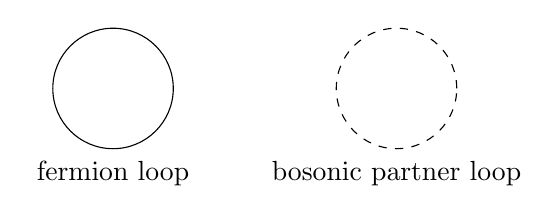
\begin{tikzpicture}[scale=0.9]
\draw (-2.0,0) circle (0.85);
\draw[dashed] (2.0,0) circle (0.85);
\node at (-2.0,-1.2) {fermion loop};
\node at (2.0,-1.2) {bosonic partner loop};
\end{tikzpicture}
\caption{電荷の整合の議論の際に比較されたフェルミオンループとボソン的パートナーのループ。切り取られた外部の印は、枠だけではすべての取り付けを決定できないため再構成されていない。}
\end{figure}

\begin{classroomqa}
\audiencequestion{超対称パートナーが検出を逃れてきたのは、単にそれらの結合定数が異なるからだろうか？ \lecturetimestamp{00:56:23}}
\lecturerresponse{同じ図が相殺するのであれば、そうではない。光子相互作用を加えることは各線の電気電荷を試すことになる。等しくない結合は等しくない数値的ループ因子を与え、大きな残りを復活させる。対称性は適切な電荷と相互作用を整合させねばならない。}
\end{classroomqa}

\begin{classroomqa}
\audiencequestion{光子の超対称パートナーもまた質量ゼロであるべきだろうか？ \lecturetimestamp{00:58:01}}
\lecturerresponse{厳密な超対称理論では、光子と縮退しているため質量ゼロとなるであろう。観測される世界は厳密には超対称ではないので、物理的なフォティーノ的な状態が光子と同じ質量を共有する必要はない。}
\end{classroomqa}

\section{超対称パートナー対応表}

命名規則は洗練されていないが有用である。ボソンはフェルミオン的パートナーを受け取り、その名前はしばしば\emph{-イーノ}で終わる：光子とフォティーノ、\(W\)とウィーノ、\(Z\)とジーノ、グルーオンとグルイーノ、ヒッグスとヒッグシーノ、グラビトンとグラビティーノ。通常のフェルミオンはボソン的パートナーを受け取り、その名前は通常\emph{s-}で始まる：電子とセレクトロン、クォークとスクォーク。

\begin{center}
\begin{tabular}{@{}>{\raggedright\arraybackslash}p{0.40\linewidth}>{\raggedright\arraybackslash}p{0.52\linewidth}@{}}
\toprule
通常の状態 & 超対称パートナーとスピン変化\\
\midrule
スカラーヒッグス、\(j=0\) & ヒッグシーノ、\(j=\tfrac12\)；\(\Delta j=+\tfrac12\)\\
ゲージボソン、\(j=1\) & ゲージーノ、\(j=\tfrac12\)；\(\Delta j=-\tfrac12\)\\
物質フェルミオン、\(j=\tfrac12\) & スフェルミオン、\(j=0\)；\(\Delta j=-\tfrac12\)\\
グラビトン、\(j=2\) & グラビティーノ、\(j=\tfrac32\)；\(\Delta j=-\tfrac12\)\\
\bottomrule
\end{tabular}
\end{center}

一般的な関係は、超多重項のメンバーはスピンの半単位だけ異なるということである：
\begin{equation}
\Delta j=\frac12.
\end{equation}
講義の大まかな例では、スピン\(\tfrac12\)の物質フェルミオンをスカラーと対にし、スピン1のゲージボソンをスピン\(\tfrac12\)のゲージーノと対にする。完全な相互作用模型では対称性の破れ後に状態が混合しうるので、物理的な質量固有状態がこれらの最も単純な名前を保持する必要はない。

\begin{classroomqa}
\audiencequestion{新しいスカラーパートナーがすべて独自の自発的対称性の破れを起こすことはありうるだろうか？ \lecturetimestamp{01:01:27}}
\lecturerresponse{スカラー場は期待値を獲得しうるが、任意の余分な対称性の破れは現象論的に破滅的であろう。実行可能な超対称模型は、カラー、電荷、その他の必要な対称性が誤った形で破られないようにスカラーポテンシャルを整えなければならない。}
\end{classroomqa}

\begin{classroomqa}
\audiencequestion{ヒッグシーノはヒッグスの四重項項に対応する特別な相互作用を持つだろうか？ \lecturetimestamp{01:02:19}}
\lecturerresponse{超対称性は粒子だけでなく相互作用も対応させる。この関係はすべてのヒッグス線をヒッグシーノ線に素朴に置き換えることによって得られるのではないが、スカラー四重項と関連するフェルミオン的および補助的相互作用は一つの拘束された構造に属する。それらの詳細は講義ではまだ展開されていない。}
\end{classroomqa}

\begin{classroomqa}
\audiencequestion{\(2\pi\)対\(4\pi\)回転定理には他の次元における類似物があるだろうか？ \lecturetimestamp{01:03:07}}
\lecturerresponse{はい、しかし次元性が可能性を変える。二つの空間次元では交換経路が互いの周りを巻きつくことができ、交換位相がボソン的\(+1\)やフェルミオン的\(-1\)よりも一般的であるエニオンを許す。そのような励起は凝縮系で生じるが、それらは本講義の経路の外にある。}
\end{classroomqa}

\section{なぜ厳密な超対称性は化学を消し去るか}

最後に、厳密に超対称な世界がどのようなものであるかを問う。ここで厳密とは、すべての粒子-超対称パートナー対について質量が等しく相互作用が対応していることを意味する。電子は同じ質量と電荷を持つボソン的セレクトロンを持ち、質量ゼロの光子は質量ゼロのフェルミオン的フォティーノを持つであろう：
\begin{equation}
m_{\widetilde e}=m_e,
\qquad
q_{\widetilde e}=q_e,
\qquad
m_{\widetilde\gamma}=m_\gamma=0.
\end{equation}

化学のよく知られた周期構造はフェルミ統計に依存する。水素は最低軌道に一つの電子を持つ。ヘリウムはスピンラベルが異なるためそこに二つを収容する。リチウムの第三の電子はより高い軌道を占めなければならない：パウリの排他原理は三つの同一の電子が同じ一粒子状態を占めることを妨げる。その外側の電子はより多くのエネルギーを持ち、通常は光子を放出して内側に落ち込みたいと望むが、満たされた低い状態がその遷移を妨げる。

厳密な超対称性は別のチャネルを開く：
\begin{equation}
e^-_{\mathrm{outer}}
\longrightarrow
\widetilde e^-_{\mathrm{inner}}
+
\widetilde\gamma .
\end{equation}
初期の電子と放出されたフォティーノはフェルミオンであり、残ったセレクトロンはボソンである。セレクトロンはフェルミ統計ではなくボース統計に従うので、最終的なセレクトロンはすでに占められた低い軌道から排除されない。したがって価電子は変換して内側に落ち込むことができる。

\begin{figure}[H]
\centering
\includegraphics[width=0.62\textwidth]{lecture_02_figure_06.png}
\lectureframe{01:09:18}

\medskip
\begin{tikzpicture}[scale=0.9]
\fill (0,0) circle (0.075);
\draw (0,0) circle (0.72);
\draw (0,0) circle (1.45);
\draw[-{Latex[length=2.2mm]}] (1.42,0.2) .. controls (1.2,0.52) and (0.92,0.42) .. (0.72,0.1);
\draw[decorate,decoration={snake,amplitude=1.4pt,segment length=7pt},-{Latex[length=2.2mm]}]
  (1.58,0) -- (3.55,0);
\node[above] at (2.7,0.12) {$\widetilde\gamma$};
\node[below] at (0,-1.65) {selectron drops to a lower orbital};
\end{tikzpicture}
\caption{厳密な超対称性がなぜ化学を変えるかを示すために用いられた原子遷移。出ていく波線は可視であり、それがフォティーノであるという同定は文字起こしによる。}
\end{figure}

この点はリチウム様原子に限られたものではない。大きな原子では、化学的な多様性を生み出すのは価電子である。もしそれらが繰り返しボソン的なセレクトロンへ変換できるなら、殻を満たすのではなく、エネルギー的に利用可能な最も低い領域に密集できる。その結果は、なじみ深い価電子軌道の構造ではなく、原子核近傍に集中したボソン的集団に似たものになるだろう。方向性のある結合と部分的に満たされた殻から作られる分子は、認識できる形では存続しないであろう。講義では、仮想的なリチウムの子孫を\emph{slithium}と呼ぶが、この冗談には深刻な結論が伴う。厳密な超対称性は、通常の化学とは異なり、したがって通常の生物学とも異なる物質を生み出すであろう。

\begin{classroomqa}
\audiencequestion{電子からセレクトロンへの遷移は、通常の原子が存続するほど弱く結合しているのだろうか。\lecturetimestamp{01:10:23}}
\lecturerresponse{ここで想定している厳密な理論ではそうではない。超対称性はこの遷移を電磁相互作用と関係づけるので、その結合は自由に微小に選ばれるのではなく、電荷によって固定される。講義では、リチウム様原子に対してマイクロ秒程度の粗い寿命が与えられる。これは精密計算としてではなく、崩壊が急速であろうことを強調するためである。}
\end{classroomqa}

したがって、衝突型加速器による探索とはまったく別に、日常的な物質から、超対称性が低エネルギーで厳密ではありえないことがわかる。粒子と超対称パートナーの質量の隔たりは、原子や陽子のスケールと比べて莫大である。たとえ統一スケールやプランクスケールと比べれば小さくても、である。

\begin{classroomqa}
\audiencequestion{では、なぜ超対称性は破れているのか。\lecturetimestamp{01:11:19}}
\lecturerresponse{講義は最小限の選択の言明を提示する。もし破れていなければ、通常の化学から構成された観測者は、この問いを発するために存在しないであろう。これは超対称性の破れの力学理論の代わりにはならない。厳密に超対称な低エネルギーの世界がなぜ我々の世界でありえないかを説明するだけである。}
\end{classroomqa}

超対称性を破ることは数学的に可能であり、多くの構成ではむしろ一般的であるが、現実的な破れを整えることは決して自動的ではない。逆に、厳密に超対称な量子場の理論は、一般的な理論よりもはるかに深く解析できるほど十分な特別な構造をもつ。それらは素粒子物理学を組織する候補としても、並外れて強力な数学的実験室としても役立つ。次の講義では、この物理的動機から、その構造のさらなる部分へと移る。

\section{議論の糸}

超対称性への道は意図的に間接的であった。
\begin{enumerate}
\item \(2\pi\)の空間回転は非自明なトポロジー的類に属するが、\(4\pi\)の回転は恒等変換に変形できる。
\item フェルミオン状態は\(2\pi\)の下で負の符号を獲得し、二経路実験は、その符号が大域的ではなく相対的であるときに観測可能にする。
\item 交換の下でのフェルミオン的反対称性は、すべての閉じたフェルミオンループに、ボソンループに対する余分な負の符号を与える。
\item 逆のループ符号は、質量と結合が一致するとき、真空およびスカラー自己エネルギーの寄与が対称性によって強制される相殺を可能にする。
\item 厳密な一致は自然界には存在しない。もし超対称性がヒッグスセクターを保護するなら、その破れによって関連するパートナーを任意に重くすることはできない。
\item 厳密な低エネルギー超対称性は、電子がボソン的なセレクトロンへ変換することを許し、通常の化学が依存する殻構造を崩壊させるであろう。
\end{enumerate}

したがって超対称性が魅力的であり、かつその素朴な厳密な形では不可能であるのは、同じ理由による。すなわち、ボソンとフェルミオンを緊密に結びつけるからである。この緊密な関係は危険な量子補正を飼いならすことができるが、もしそれが破れずに原子物理学にまで生き残るなら、世界は我々の周囲の世界に似たものではなくなってしまうであろう。